\section{Multi Instance Learning}
 
\subsection*{Introduction}
\begin{frame}{Multi instance classification}
	Motivation:
	\begin{itemize}\setlength\itemsep{1em}
		\item Sometimes a complex item can be well represented by a set of \textit{features} or \textit{instances}
		\item A single instance may belong or not to a class or \textit{label} (positive or negative)
		\item An example, or \textit{bag}, is positive if at least one of its instances is positive (it is called \textit{witness}), where as a negative bag consists of only negative instances
		\item A label is provided for the
		entire bag, not to instances
		\item We have a \textit{semi-supervised learning} problem
	\end{itemize}
	\begin{flushright}
		\cite{mi1}
	\end{flushright}
\end{frame}

\begin{frame}{Notation}
	Dataset is now a set of bags, where each bag is a set of instances:
	$$D = \{(X_i, Y_i) | \ i \in [1, n]\}$$
	$$X_i = \{x_{i,k} | \ k \in [1, k_i], x_{i,k} \in \R^f\}$$
	Notice that each bag can be made of any number of instances, but every instance has a fixed number of features $f$.
	\begin{figure}[htbp]
		\centering
		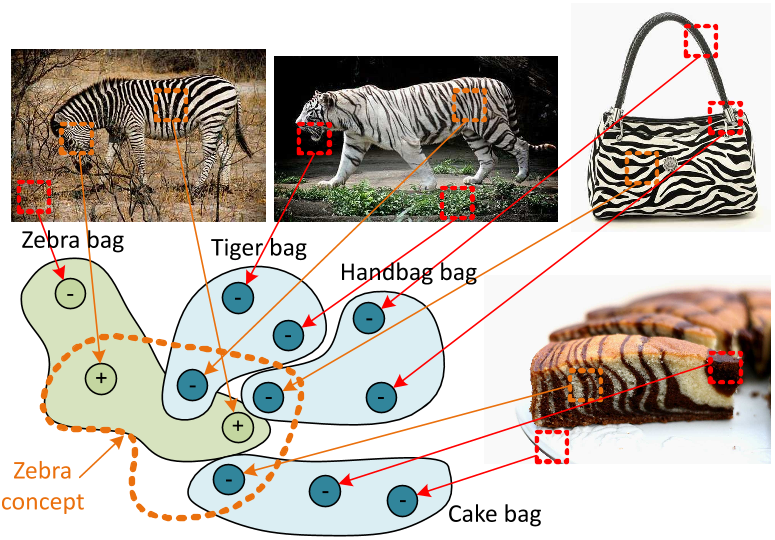
\includegraphics[scale = 0.15]{./images/mi3.png}
		\caption{\textit{Example of images instances refer to "zebra concept"}}
	\end{figure}
	\color{red}IMMAGINE MI?
\end{frame}

\subsection{SIL}
\begin{frame}{SIL}
	The first naive approach makes the following label assignment:
	\begin{itemize}\setlength\itemsep{1em}
		\item If an instance belongs to a negative bag, sets its label to $-1$
		\item If an instance belongs to a positive bag, sets its label to $+1$
	\end{itemize}
	\vspace{5px}
	The resulting problem can be solved using a regular SVM, treating each instance as a whole document.\\
	\vspace{12px}
	Using this approach makes almost useless multi-instance formulation.
\end{frame}


\subsection{mi-SVM}
\begin{frame}{mi-SVM}
	Instances label assignment:
	\begin{itemize}\setlength\itemsep{1em}
		\item If an instance belongs to a negative bag we can say that its label is $-1$
		\item If an instance belongs to a positive bag we don't know for sure its label
	\end{itemize}
	\vspace{12px}
	This leads to 2 new constraints in SVM problem:
	$$y_{i,k} = -1 \ if \ Y_i = -1$$
	$$\sum_{k = 1}^{k_i}\frac{y_{i,k} + 1}{2} \geq 1 \ if \ Y_i = +1$$
\end{frame}

\begin{frame}{mi-SVM}
	Our SVM problem becames the following:
	$$min_Y min_{w, \xi} \frac{1}{2} ||w||^2 + C \sum_{i = 1}^{n}\xi_i$$
	$$y_{i,k} (w^T x_{i,k} + b) \geq 1 - \xi_i \ \forall i \in [1, n], k \in [1, k_i]$$
	$$\xi_i \geq 0 \ \forall i \in [1, n]$$
	$$y_{i,k} = -1 \ if \ Y_i = -1$$
	$$\sum_{k = 1}^{k_i}\frac{y_{i,k} + 1}{2} \geq 1 \ if \ Y_i = +1$$
	That is an intractable mixed optimization problem
\end{frame}

\begin{frame}{mi-SVM algorithm}
	A feasible algorithm that finds a non optimal solution is the following:
	
	\begin{codebox}
		\Procname{$\proc{mi-SVM}\left(X, Y\right)$}
		\li $y_{i,k} = -1 \ if \ Y_i = -1$
		\li $y_{i,k} = +1 \ if \ Y_i = +1$
		\li \textbf{do} \Do
		\li Solve regular SVM finding $w$, $b$
		\li $y_{i,k} = sign(w^T x_{i,k} + b) \ if \ Y_i = +1$
		\li Adjust each positive bag to satisfy constraints \End
		\li \While($y_{i,k}$ change)
		
	\end{codebox}
	
\end{frame}

\subsection{MI-SVM}
\begin{frame}{MI-SVM}
	This approach uses directly the dataset in its bag form:
	$$arg min_{w, \xi} \frac{1}{2} ||w||^2 + C \sum_{i = 1}^{n}\xi_i$$
	$$y_i (max_k w^T x_{i,k} + b) \geq 1 - \xi_i \ \forall i \in [1, n]$$
	$$\xi_i \geq 0 \ \forall i \in [1, n]$$
	This is possible by selecting a \textit{witness} from each bag instance.
\end{frame}

\begin{frame}{MI-SVM algorithm}
	A feasible algorithm that finds a solution is the following:
	
	\begin{codebox}
		\Procname{$\proc{MI-SVM}\left(X, Y\right)$}
		\li $\bar{x}_i = avg(x_{i,k}) \ \forall x_{i,k} \in X_i$ positive bag
		\li \textbf{do} \Do
		\li Assign $\bar{\alpha}_i \in [0,C]$ to each $\bar{x}_i$
		\li Assign $\alpha_{i,j}$ with $\sum_{j=1}^{k_i}\alpha_{i,j} \in [0,C] \ \forall x_{i,k} \in X_i$ negative bag
		\li Solve regular SVM finding $w$, $b$
		\li Find new $\bar{x}_i$ by selecting the best one for each positive bag \End
		\li \While(witnesses change)
		
	\end{codebox}
	
\end{frame}

\begin{frame}{Other common frameworks for MI}
	In addition to these methods we can cite:
	\begin{itemize}
		\item \textbf{Diverse density (DD)}: DD COMPLICATO
		\item \textbf{EM-DD}: COMPLICATO
		\item \textbf{Citation kNN}: documento OKOK
		\item \textbf{MIL Random forest (MIL RF)}: PAGAMENTO
		\item \textbf{MBSTAR}: MicroRNA
	\end{itemize}
\end{frame}

